\usetikzlibrary{arrows.meta,calc}
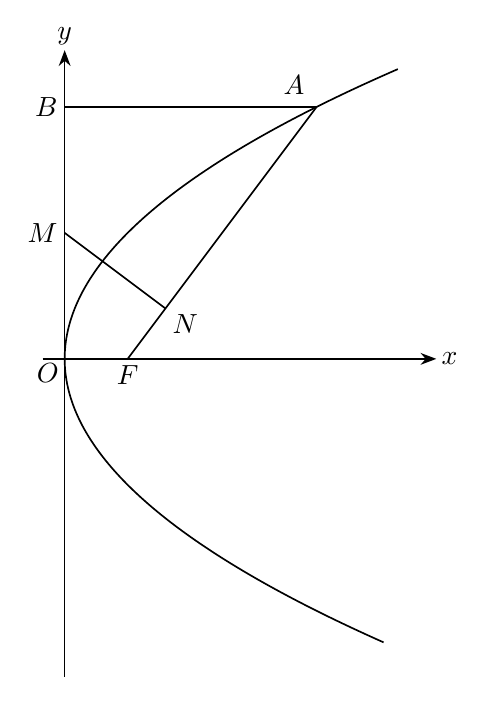
\begin{tikzpicture}[x=0.8cm,y=0.8cm,line width=.6pt,>=Stealth,font=\normalsize]
\coordinate (O) at (0,0);
\coordinate (A) at (4,4);
\coordinate (B) at (0,4);
\coordinate (M) at (0,2);
\coordinate (F) at (1,0);
\coordinate (N) at (1.6,0.8);
\draw[->] (-0.35,0)--(5.9,0);
\draw[->] (0,-5.05)--(0,4.9);
\draw[domain=-4.5:4.6,samples=181] plot ({(\x*\x)/4},{\x});
\draw (B)--(A);
\draw (F)--(A);
\draw (M)--(N);
\node[anchor=north east,inner sep=0pt] at (-0.08,-0.06) {$O$};
\node[anchor=east,inner sep=0pt] at (-0.1,4) {$B$};
\node[anchor=east,inner sep=0pt] at (-0.1,2) {$M$};
\node[anchor=south east,inner sep=0pt] at (3.82,4.18) {$A$};
\node[anchor=north,inner sep=0pt] at (1,-0.1) {$F$};
\node[anchor=north west,inner sep=0pt] at (1.7,0.72) {$N$};
\node[anchor=west,inner sep=0pt] at (5.97,0) {$x$};
\node[anchor=south,inner sep=0pt] at (0,4.97) {$y$};
\end{tikzpicture}
